\documentclass[10pt, xcolor=x11names, compress]{beamer}
%\documentclass[10pt, xcolor=x11names, compress, handout]{beamer}
\usetheme{progressbar}
%\usecolortheme[named=Purple4]{structure}
\progressbaroptions{headline=sections,titlepage=normal,frametitle=normal}

\setbeamertemplate{navigation symbols}{}

\usepackage{iwona} 

\usepackage{alltt}
\usepackage{amsmath,amsfonts, amssymb, amscd}
\usepackage{hyperref}
\usepackage{setspace}
\usepackage{wasysym}
\usepackage{ulem}

\usepackage{calc}
\usepackage[overlay,absolute]{textpos}
\TPGrid[5mm,5mm]{20}{20}



\renewcommand{\Re}{\operatorname{Re}}
\renewcommand{\Im}{\operatorname{Im}}
\newcommand{\debye}{\operatorname{debye}}

\newcommand{\chik}{$\chi(k)$}
\newcommand{\chir}{$|\tilde{\chi}(R)|$}


\newcommand{\file}[1]{{\color{Firebrick4}\texttt{`#1'}}}
\newcommand{\multiple}{{\color{Orange3}\textsl{multiple}}}


\newcommand{\atoms}  {{\color{DarkOrchid4}\textsc{atoms}}}
\newcommand{\feff}   {{\color{DarkOrchid4}\textsc{feff}}}
\newcommand{\ifeffit}{{\color{DarkOrchid4}\textsc{ifeffit}}}
\newcommand{\athena} {{\color{DarkOrchid4}\textsc{athena}}}
\newcommand{\artemis}{{\color{DarkOrchid4}\textsc{artemis}}}

\renewenvironment<>{center}
{\begin{actionenv}#1\begin{originalcenter}}
{\end{originalcenter}\end{actionenv}}

\definecolor{guessp}   {rgb}{0.64,0.00,0.64}
\newcommand{\guessp}   {{\color{guessp}guess}}
\definecolor{defp}     {rgb}{0.00,0.55,0.00}
\newcommand{\defp}     {{\color{defp}def}}
\definecolor{setp}     {rgb}{0,0,0}
\newcommand{\setp}     {{\color{setp}set}}
\definecolor{lguessp}  {rgb}{0.24,0.11,0.56}
\newcommand{\lguessp}  {{\color{lguessp}lguess}}
\definecolor{skipp}    {rgb}{0.70,0.70,0.70}
\newcommand{\skipp}    {{\color{skipp}skip}}
\definecolor{restrainp}{rgb}{0.80,0.61,0.11}
\newcommand{\restrainp}{{\color{restrainp}restrain}}
\definecolor{afterp}   {rgb}{0.29,0.44,0.55}
\newcommand{\afterp}   {{\color{afterp}after}}
\definecolor{penaltyp} {rgb}{0.55,0.35,0.17}
\newcommand{\penaltyp} {{\color{penaltyp}penalty}}
\definecolor{mergep}   {rgb}{0.93,0.00,0.00}
\newcommand{\mergep}   {{\color{mergep}merge}}

\usepackage{chemfig}
\usepackage{mol2chemfig}

%% define new commands here
%\newcommand{\eto}{EuTiO$_3$}

%% this makes the dashed lines to the Hg atoms
\newcommand*{\bondwidth}{0.17 em} %'Bond Width'
\newcommand*{\bondboldwidth}{0.22832 em} %'Bold Width'
\newcommand*{\bondhashlength}{0.25737 em} % 'Hash Spacing'
\tikzset{
  bold bond/.style = {line width = \bondboldwidth},
  dash bond/.style =
    {dash pattern = on \bondhashlength off \bondhashlength},
  hash bond/.style =
    {
      dash pattern = on \bondwidth off \bondhashlength,
      line width   = \bondboldwidth
    },
}

\newcommand{\qm}{?}
\newcommand{\spc}{~}

\newcommand\namebond[4][5pt]{\chemmove{\path(#2)--(#3)node[midway,sloped,yshift=#1]{#4};}}
\newcommand\arcbetweennodes[3]{%
  \pgfmathanglebetweenpoints{\pgfpointanchor{#1}{center}}{\pgfpointanchor{#2}{center}}%
  \let#3\pgfmathresult}
\newcommand\arclabel[6][stealth-stealth,shorten <=1pt,shorten >=1pt]{%
  \chemmove{%
    \arcbetweennodes{#4}{#3}\anglestart \arcbetweennodes{#4}{#5}\angleend
    \draw[#1]([shift=(\anglestart:#2)]#4)arc(\anglestart:\angleend:#2);
    \pgfmathparse{(\anglestart+\angleend)/2}\let\anglestart\pgfmathresult
    \node[shift=(\anglestart:#2+4pt)#4,anchor=\anglestart+180,rotate=\anglestart+90,inner sep=0pt,
    outer sep=0pt]at(#4){#6};}}




\mode<presentation>

\title{A challenging EXAFS analysis problem}
%\subtitle{}

\author{Bruce Ravel}
\institute[NIST]{Synchrotron Methods Group, Materials Measurement Science Division\\%
  Materials Measurement Laboratory\\%
  National Institute of Standards and Technology\\%
  \&\\%
  Local Contact, Beamline X23A2\\%
  National Synchrotron Light Source\\~}


%\date[Diamond2011]{EXAFS Data Analysis workshop 2011\\
  Diamond Light Source\\November 14--17, 2011\\~}

\date[ACXAS 2014]{ASEAN Workshop on X-ray Absorption Spectroscopy\\
  Synchrotron Light Research Institute\\June 2--4, 2014}

\begin{document}
\maketitle

\begin{frame}
  \frametitle{Copyright}
  \tiny

  This document is copyright \copyright 2007-2010 Bruce Ravel.

  \begin{center}
    
\includegraphics[width=1.0cm]{images/somerights20}
  \end{center}

  This work is licensed under the Creative Commons
  Attribution-ShareAlike License.  To view a copy of this license,
  visit \href{http://creativecommons.org/licenses/by-sa/3.0/}
  {\color{Purple4}\texttt{http://creativecommons.org/licenses/by-sa/3.0/}}
  or send a letter to Creative Commons, 559 Nathan Abbott Way,
  Stanford, California 94305, USA.

  \begin{description}
  \item[You are free:] %
    \begin{itemize}
    \item \textbf{to Share} --- to copy, distribute, and transmit the work
    \item \textbf{to Remix} --- to adapt the work
    \end{itemize}
  \item[Under the following conditions:] %
    \begin{itemize}
    \item Attribution. You must attribute the work in the manner
      specified by the author or licensor (but not in any way that
      suggests that they endorse you or your use of the work).
    \item Share Alike. If you alter, transform, or build upon this
      work, you may distribute the resulting work only under the same,
      similar or a compatible license.
    \item Any of these conditions can be waived if you get permission
      from the author.
    \end{itemize}
  \end{description}
  \begin{itemize}
  \item For any reuse or distribution, you must make clear to others
    the license terms of this work. The best way to do this is with a
    link to the URL for this document.
  \item Any of the above conditions can be waived if you get
    permission from the copyright holder.
  \item Nothing in this license impairs or restricts the author's
    moral rights.
  \end{itemize}

  Your fair dealing and other rights are in no way affected by the
  above.  This is a human-readable summary of the Legal Code (the full
  license).


\end{frame}

%%% Local Variables:
%%% mode: latex
%%% TeX-master: "pimst2"
%%% End:


\section{Metal sensors}

\begin{frame}
  \frametitle{Transport of metal contaminants in the environment}

  \begin{columns}
    \begin{column}{0.5\linewidth}
      There are numerous natural and man-made point sources of toxic
      metals which find their way into water systems used for human
      and agricultural applications.
    \end{column}
    \begin{column}{0.5\linewidth}
      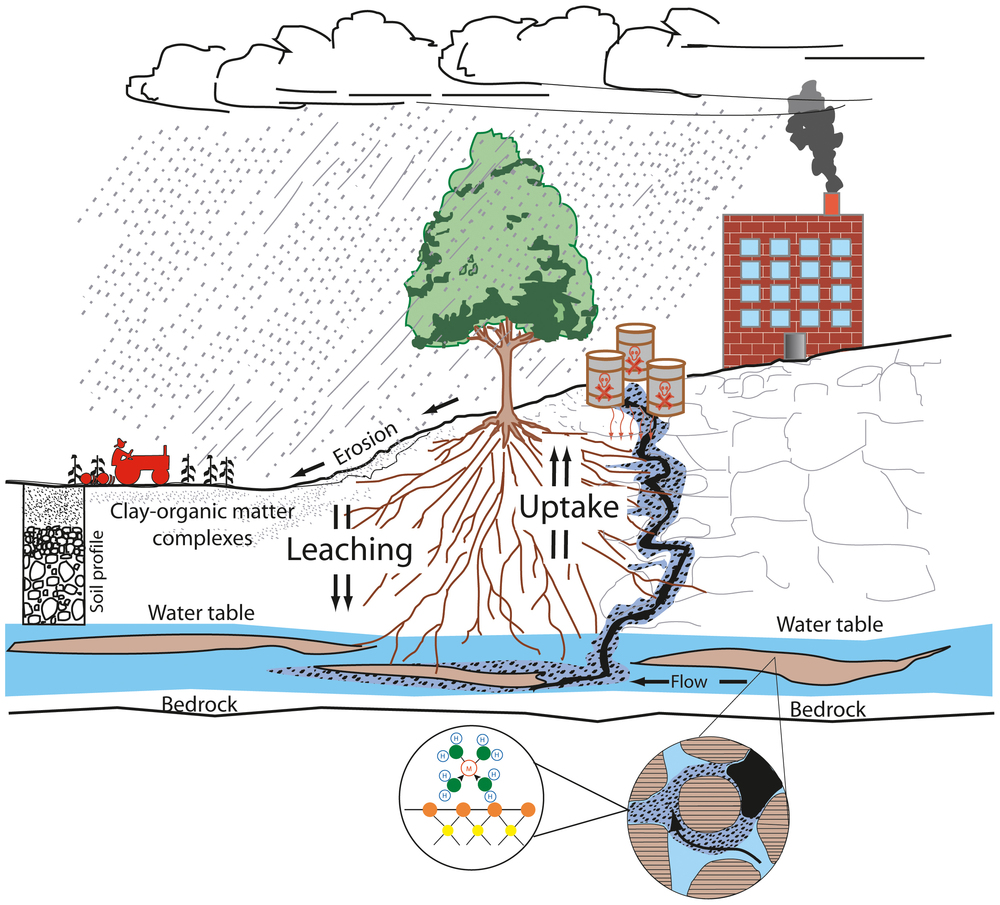
\includegraphics[width=\linewidth]{images/APS016h_sm.jpg}      
    \end{column}
  \end{columns}

  \bigskip

  \begin{exampleblock}{}
    \begin{center}
      The safe use of water requires \alert{monitoring} and eventual
      remediation of bioavailable metal species.
    \end{center}
  \end{exampleblock}

  \begin{textblock*}{0.7\linewidth}(0pt,19.5\TPVertModule)
    \tiny image from \href{http://lightsources.org}
    {\color{Blue4}\texttt{http://lightsources.org}},
    Credit: Argonne National Laboratory
  \end{textblock*}
\end{frame}

\begin{frame}
  \frametitle{Real-time, field-ready sensors}

  Sophisticated laboratory and synchrotron methods exist to detect
  and speciate water contaminants at very low concentrations.  The
  real-world task of environmental monitoring requires a
  fast, flexible, sensitive, selective method of detecting
  contaminants \alert{in the field}.

  \medskip

  \begin{columns}[T]
    \begin{column}{0.25\linewidth}<2>
      \begin{center}
        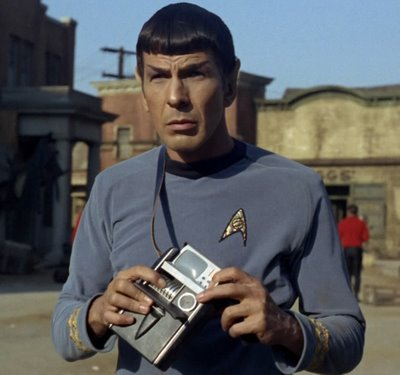
\includegraphics[width=1.1\linewidth]{images/spock+tricorder.jpg}\\
        \small We want Spock's tricorder!
      \end{center}
    \end{column}
    \begin{column}{0.75\linewidth}
      \begin{description}
      \item[Fast] Obtain results while still in the field
      \item[Flexible] Easy to carry and easy to use in the field
      \item[Sensitive] Detect contaminant concentrations below
        regulated human health hazard levels
      \item[Selective] Respond to the target metal but not to other
        metals
      \end{description}
    \end{column}
  \end{columns}
\end{frame}

\begin{frame}
  \frametitle{Catalytic DNA-based sensors}

  \begin{center}
    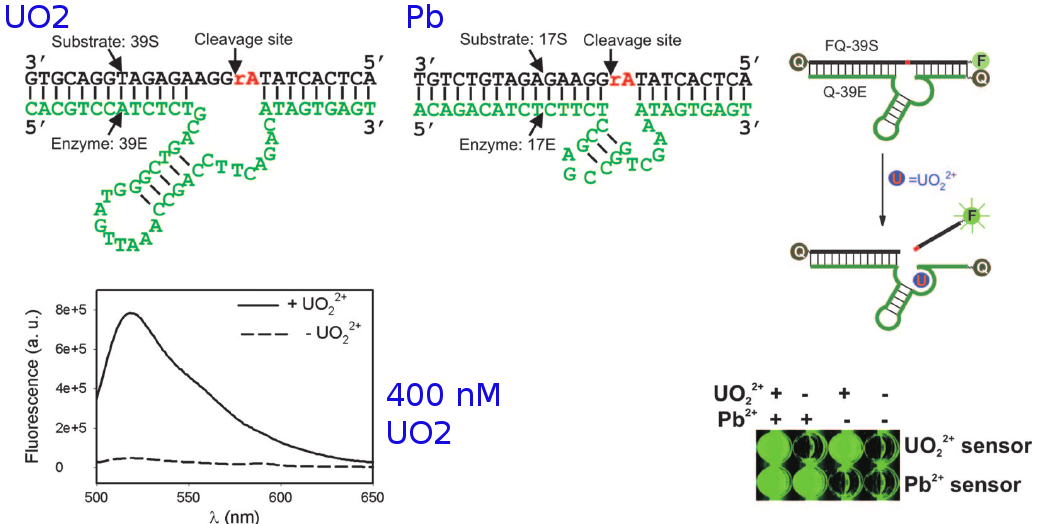
\includegraphics[width=0.8\linewidth]{images/sensor.png}
  \end{center}

  \medskip

  The sensor has a {\color{Green4}receptor}, a {\color{red}cleavage
    site}, and paired fluorophore and quencher.

  \begin{textblock*}{0.7\linewidth}(0pt,19.5\TPVertModule)%%
    \tiny J. Liu, et al. \textit{A catalytic beacon sensor for uranium
      with parts-per-trillion sensitivity and millionfold selectivity}
    PNAS, 104:7 (2007) 2056-2061
    \href{http://dx.doi.org/10.1073/pnas.0607875104}{\color{Blue4}DOI: 10.1073/pnas.0607875104}
  \end{textblock*}
\end{frame}

\begin{frame}
  \frametitle{Building a sensor device}
  \begin{center}
    These DNA sensors can be incorporated into a hand-held device.
    Water is dropped onto an array of sensors and read using
    photodiodes.

    \bigskip

    \begin{columns}
      \begin{column}{0.5\linewidth}
        \begin{center}
          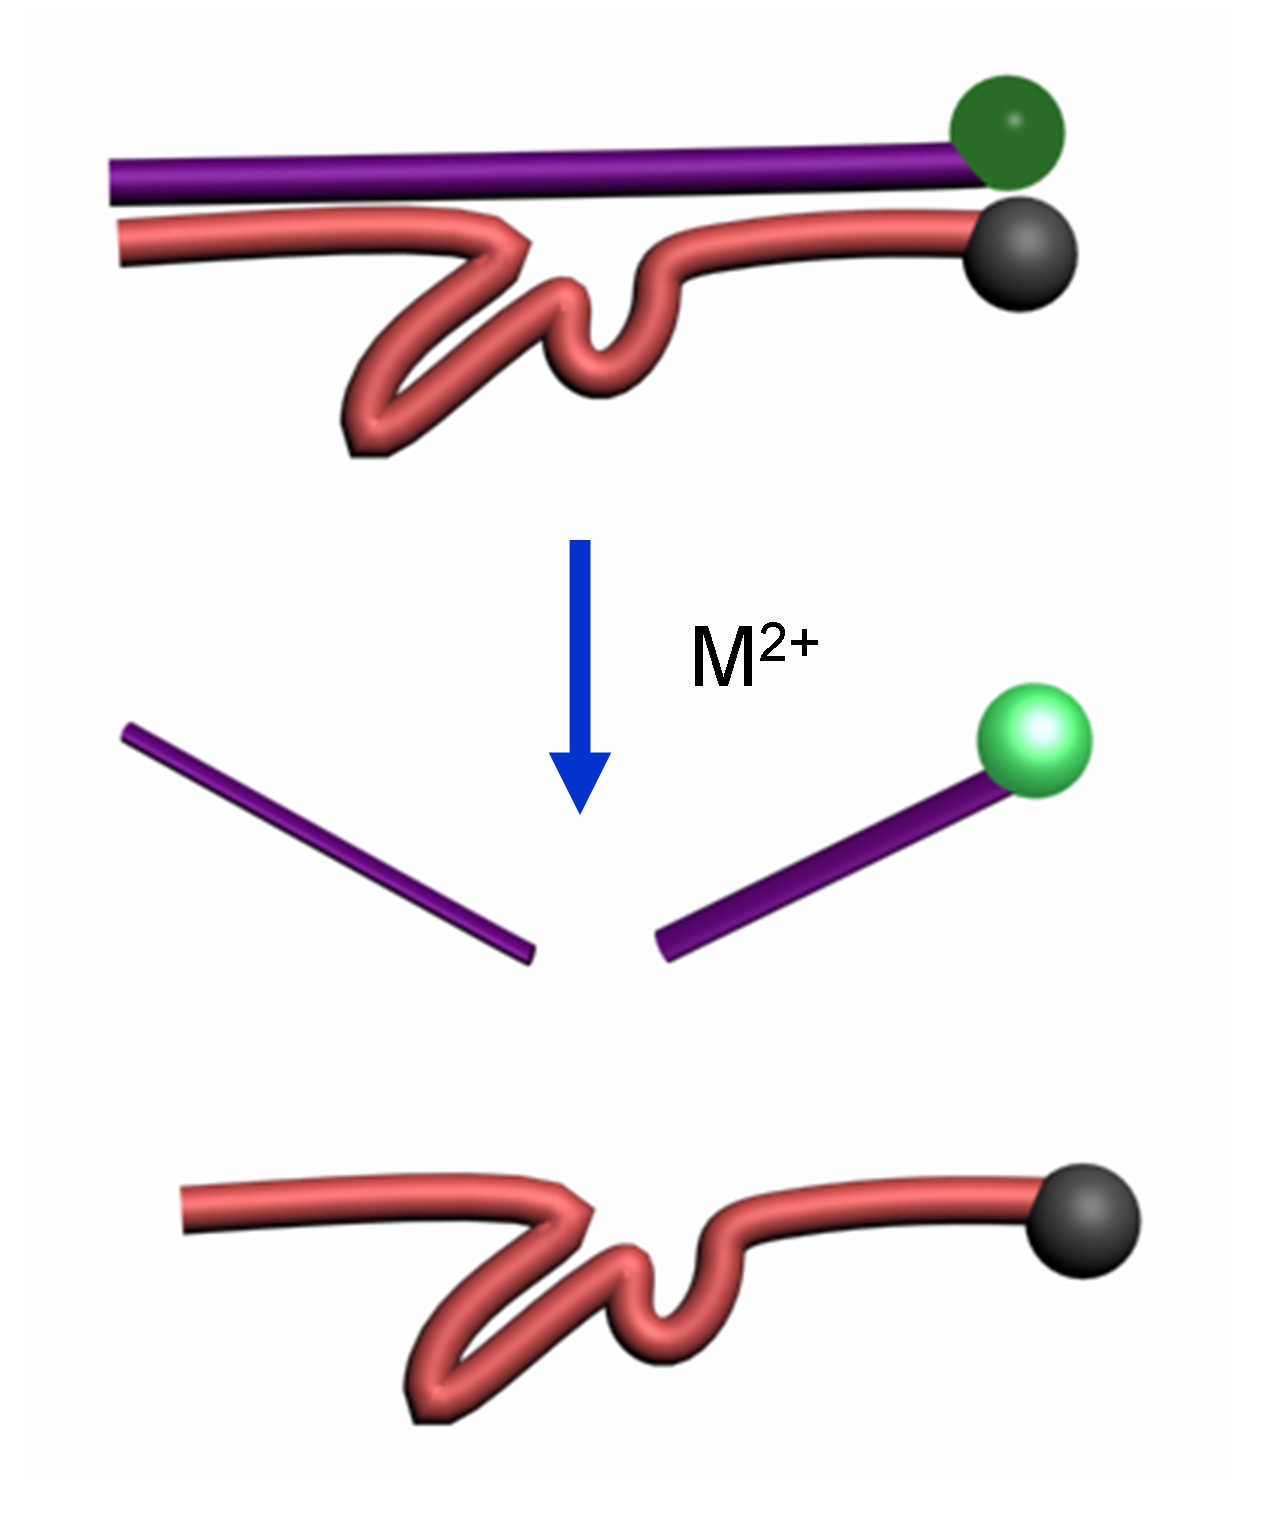
\includegraphics[width=0.8\linewidth]{images/DNAzyme_cleavage.png}
        \end{center}
      \end{column}
      \begin{column}{0.5\linewidth}
        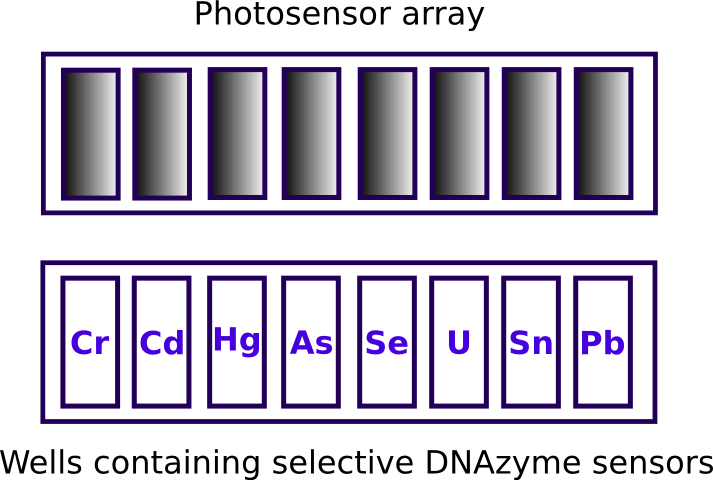
\includegraphics[width=\linewidth]{images/schematic.png}
      \end{column}
    \end{columns}

  \end{center}
\end{frame}

\section{Hg sensor}


\begin{frame}
  \frametitle{DNA-based Hg sensor}
  
  \begin{block}{U.S.\ limit on Hg in water is 10\,nM (2\,ppb)}
    The DNA-based sensor for Hg has a detection limit of 2.4\,nM
  \end{block}

  Questions:
  \begin{itemize}
  \item How and where does the metal bind?
  \item Under what conditions does the metal remain bound to the
    DNA?
  \item How many binding sites are there on a sensor?
  \item Do different metals behave differently?
  \item Can DNAzymes be designed more rationally?
  \item And, of course, what can XAS tell us about any of these
    questions (keeping in mind the very local nature of the XAS
    measurement)?
  \end{itemize}


  \begin{textblock*}{0.7\linewidth}(0pt,19\TPVertModule)%%
    \tiny J.\ Liu and Y.\ Lu. \textit{Rational Design of ``Turn-On''
      Allosteric DNAzyme Catalytic Beacons for Aqueous Mercury Ions
      with Ultrahigh Sensitivity and Selectivity}, Angew. Chemie,
    \textbf{46}:40 (2007) 7587--7590
    \href{http://dx.doi.org/10.1002/anie.200702006}{\color{Blue4}DOI:
      10.1002/anie.200702006}
  \end{textblock*}
\end{frame}

\begin{frame}
  \frametitle{XAS measurements}
  Solutions:
  \begin{itemize}
  \item 50\,mM \alert{cacodylic acid} as a buffer
  \item 100\,mM NaClO$_4$ to maintain pH=6.10
  \item glycerol to promote glassification upon freezing
  \end{itemize}

  \bigskip

  Samples:
  \begin{description}[~~~Control]
  \item[~~~Control] 15\,mM Hg
  \item[~~~Sample] 3\,mM Hg with 3\,mM DNA
  \item[~~~Sample with excess Hg] 6\,mM Hg with 3\,mM DNA
  \end{description}

  \bigskip

  \begin{block}{}
    \centering Measure EXAFS at 10\,K
  \end{block}
\end{frame}

\begin{frame}
  \frametitle{Cryostat}
  \begin{columns}
    \begin{column}{0.5\linewidth}
      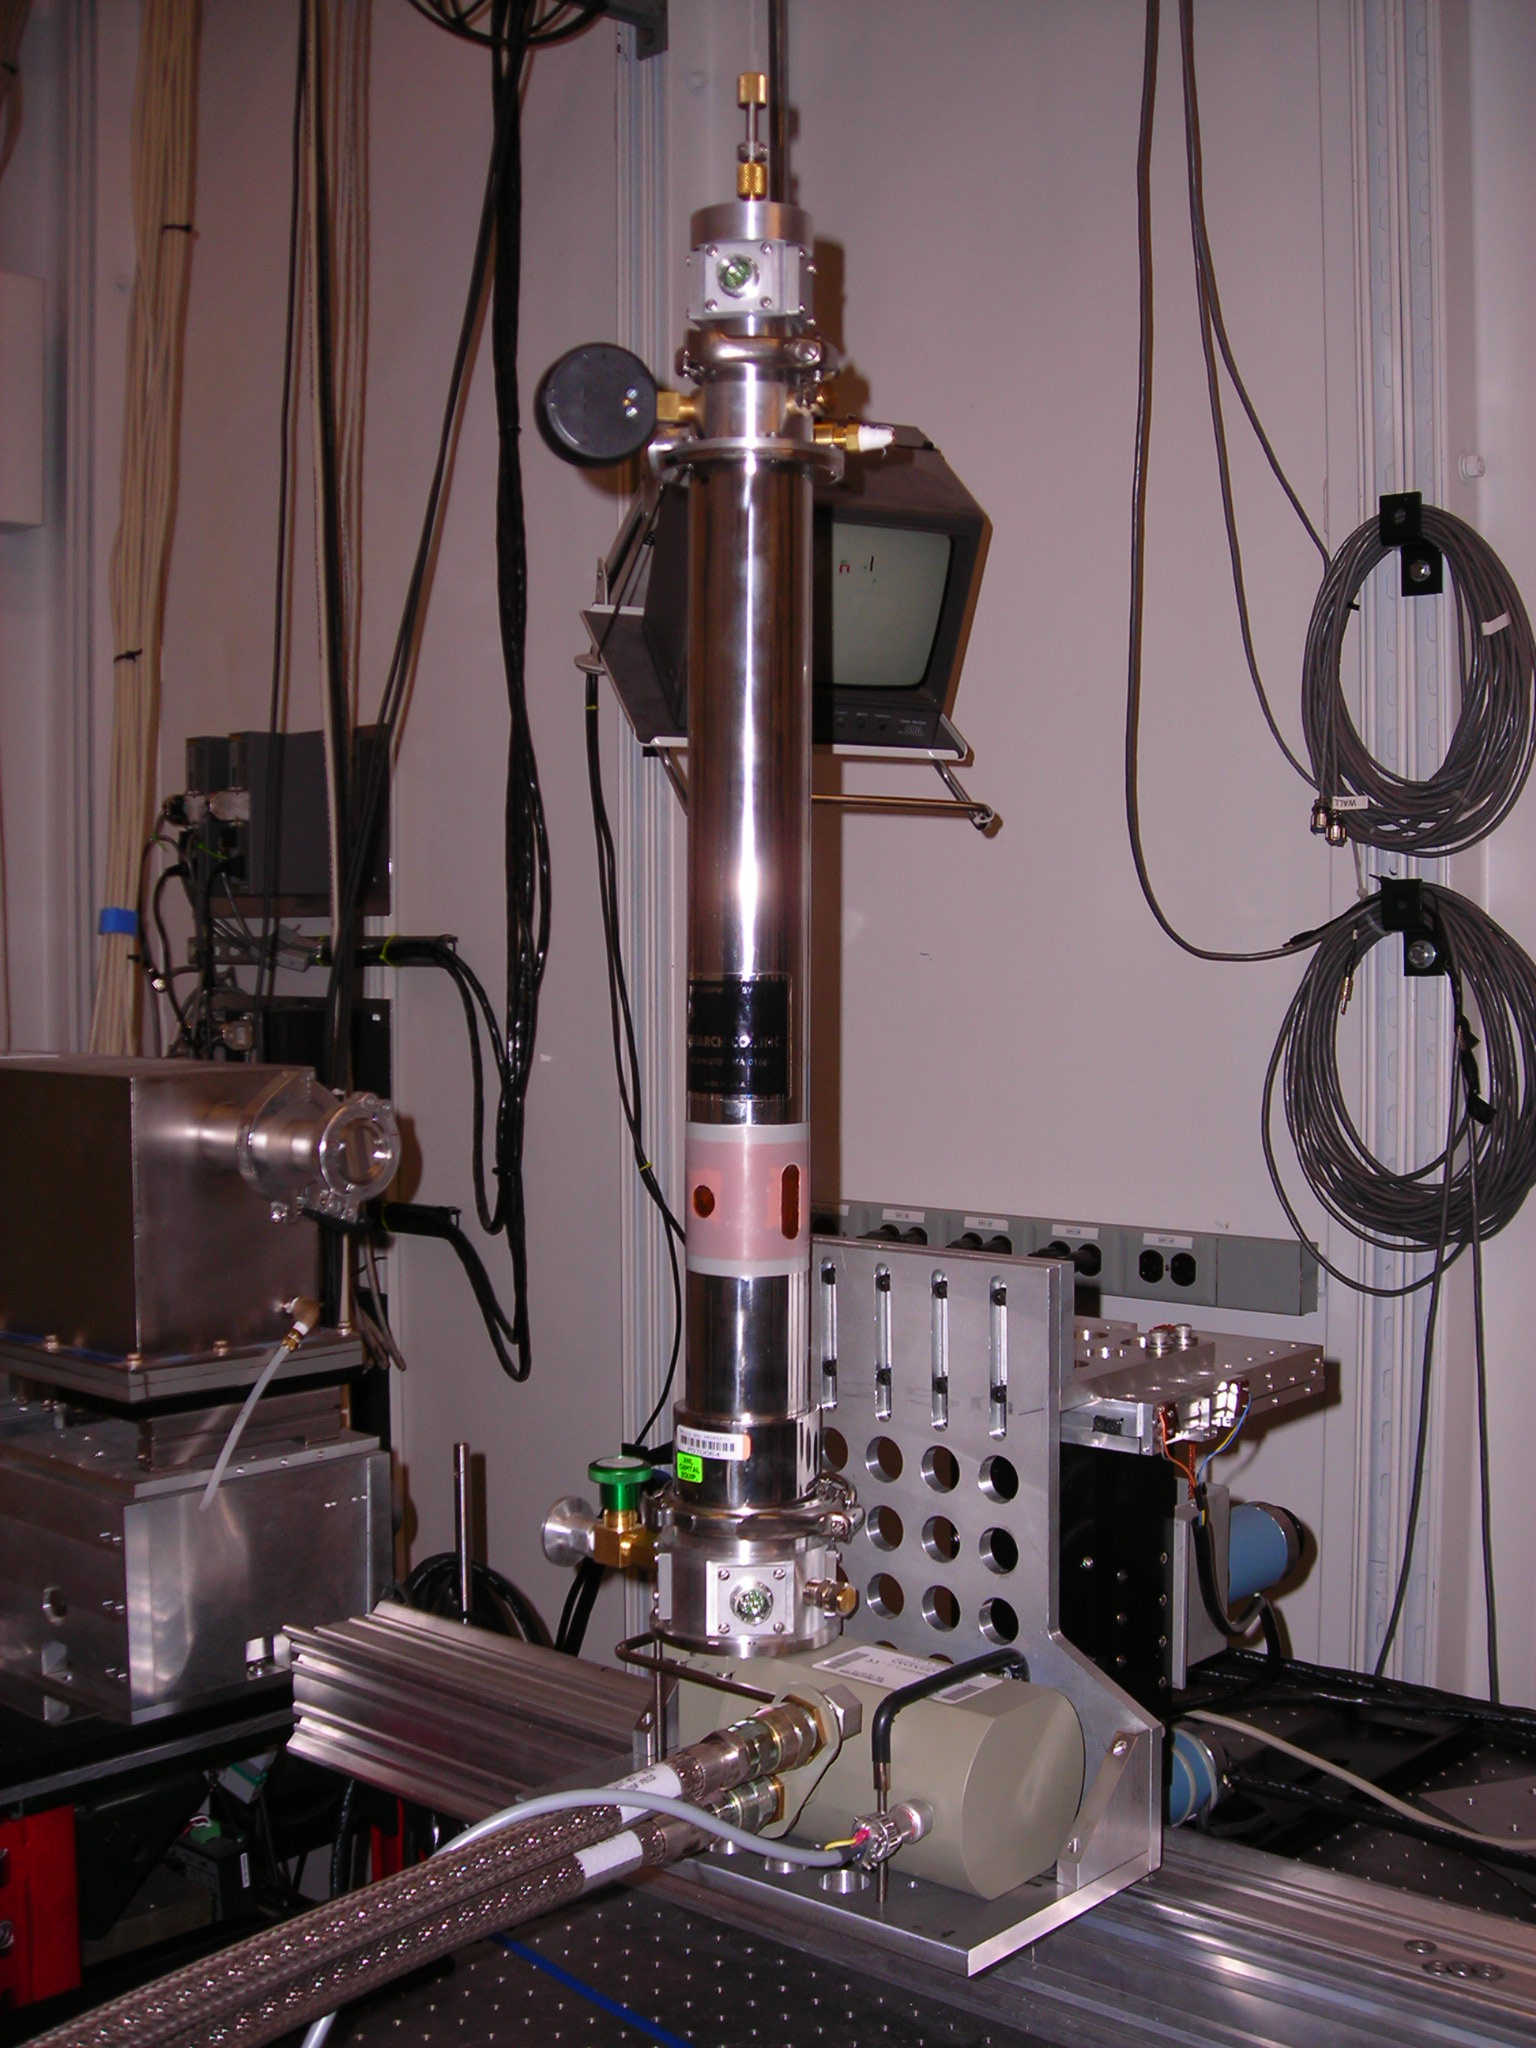
\includegraphics[width=0.8\linewidth]{images/displex.jpg}
    \end{column}
    \begin{column}{0.5\linewidth}
      Displex cryostat at APS 20BM.

      \medskip

      \begin{itemize}
      \item He exchange gas
      \item 10\,mm wide opening for beam
      \item \alert{$\sim$12\,mm wide inner shroud}
      \item Fluorescence measured through hole on side with a Ge detector
      \item At that time, 20BM did \textit{not} have a focusing mirror
      \end{itemize}
    \end{column}
  \end{columns}
\end{frame}

\begin{frame}
  \frametitle{Unforced error \#1}
  

  \begin{columns}
    \begin{column}{0.5\linewidth}
      Here is the fluorescence spectrum:\\[1ex]
      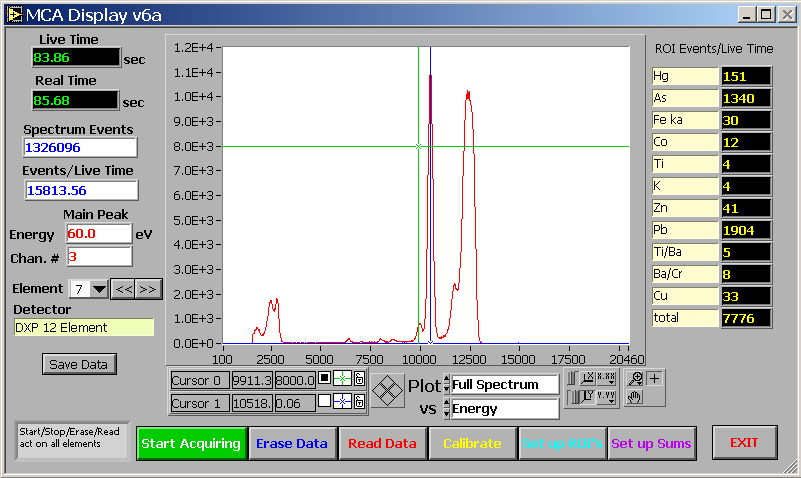
\includegraphics[width=\linewidth]{images/spectrum.png}\\[1ex]
      The Hg L$\alpha$ peak is the tiny thing near the green
      line.\\[1ex]
      The neighboring peak is vastly larger!
    \end{column}
    \begin{column}{0.5\linewidth}

      \begin{alertblock}<2-3>{}
        \centering What's cacodylic acid?
      \end{alertblock}

      \begin{center}
        \visible<3>{
          Wikipedia tells me that cacodylic acid is:

          \medskip

          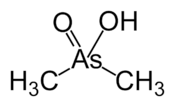
\includegraphics[width=0.35\linewidth]{images/cacodylate.png}

          \medskip

          \small
          The big peak is As K$\alpha$ ($\sim$10.5\,keV), our
          Hg L$\alpha$ ($\sim$10\,keV) peak is on its shoulder.
        }
      \end{center}
    \end{column}
  \end{columns}

\end{frame}

\begin{frame}
  \frametitle{Unforced error \#2}
  \begin{columns}
    \begin{column}{0.5\linewidth}
      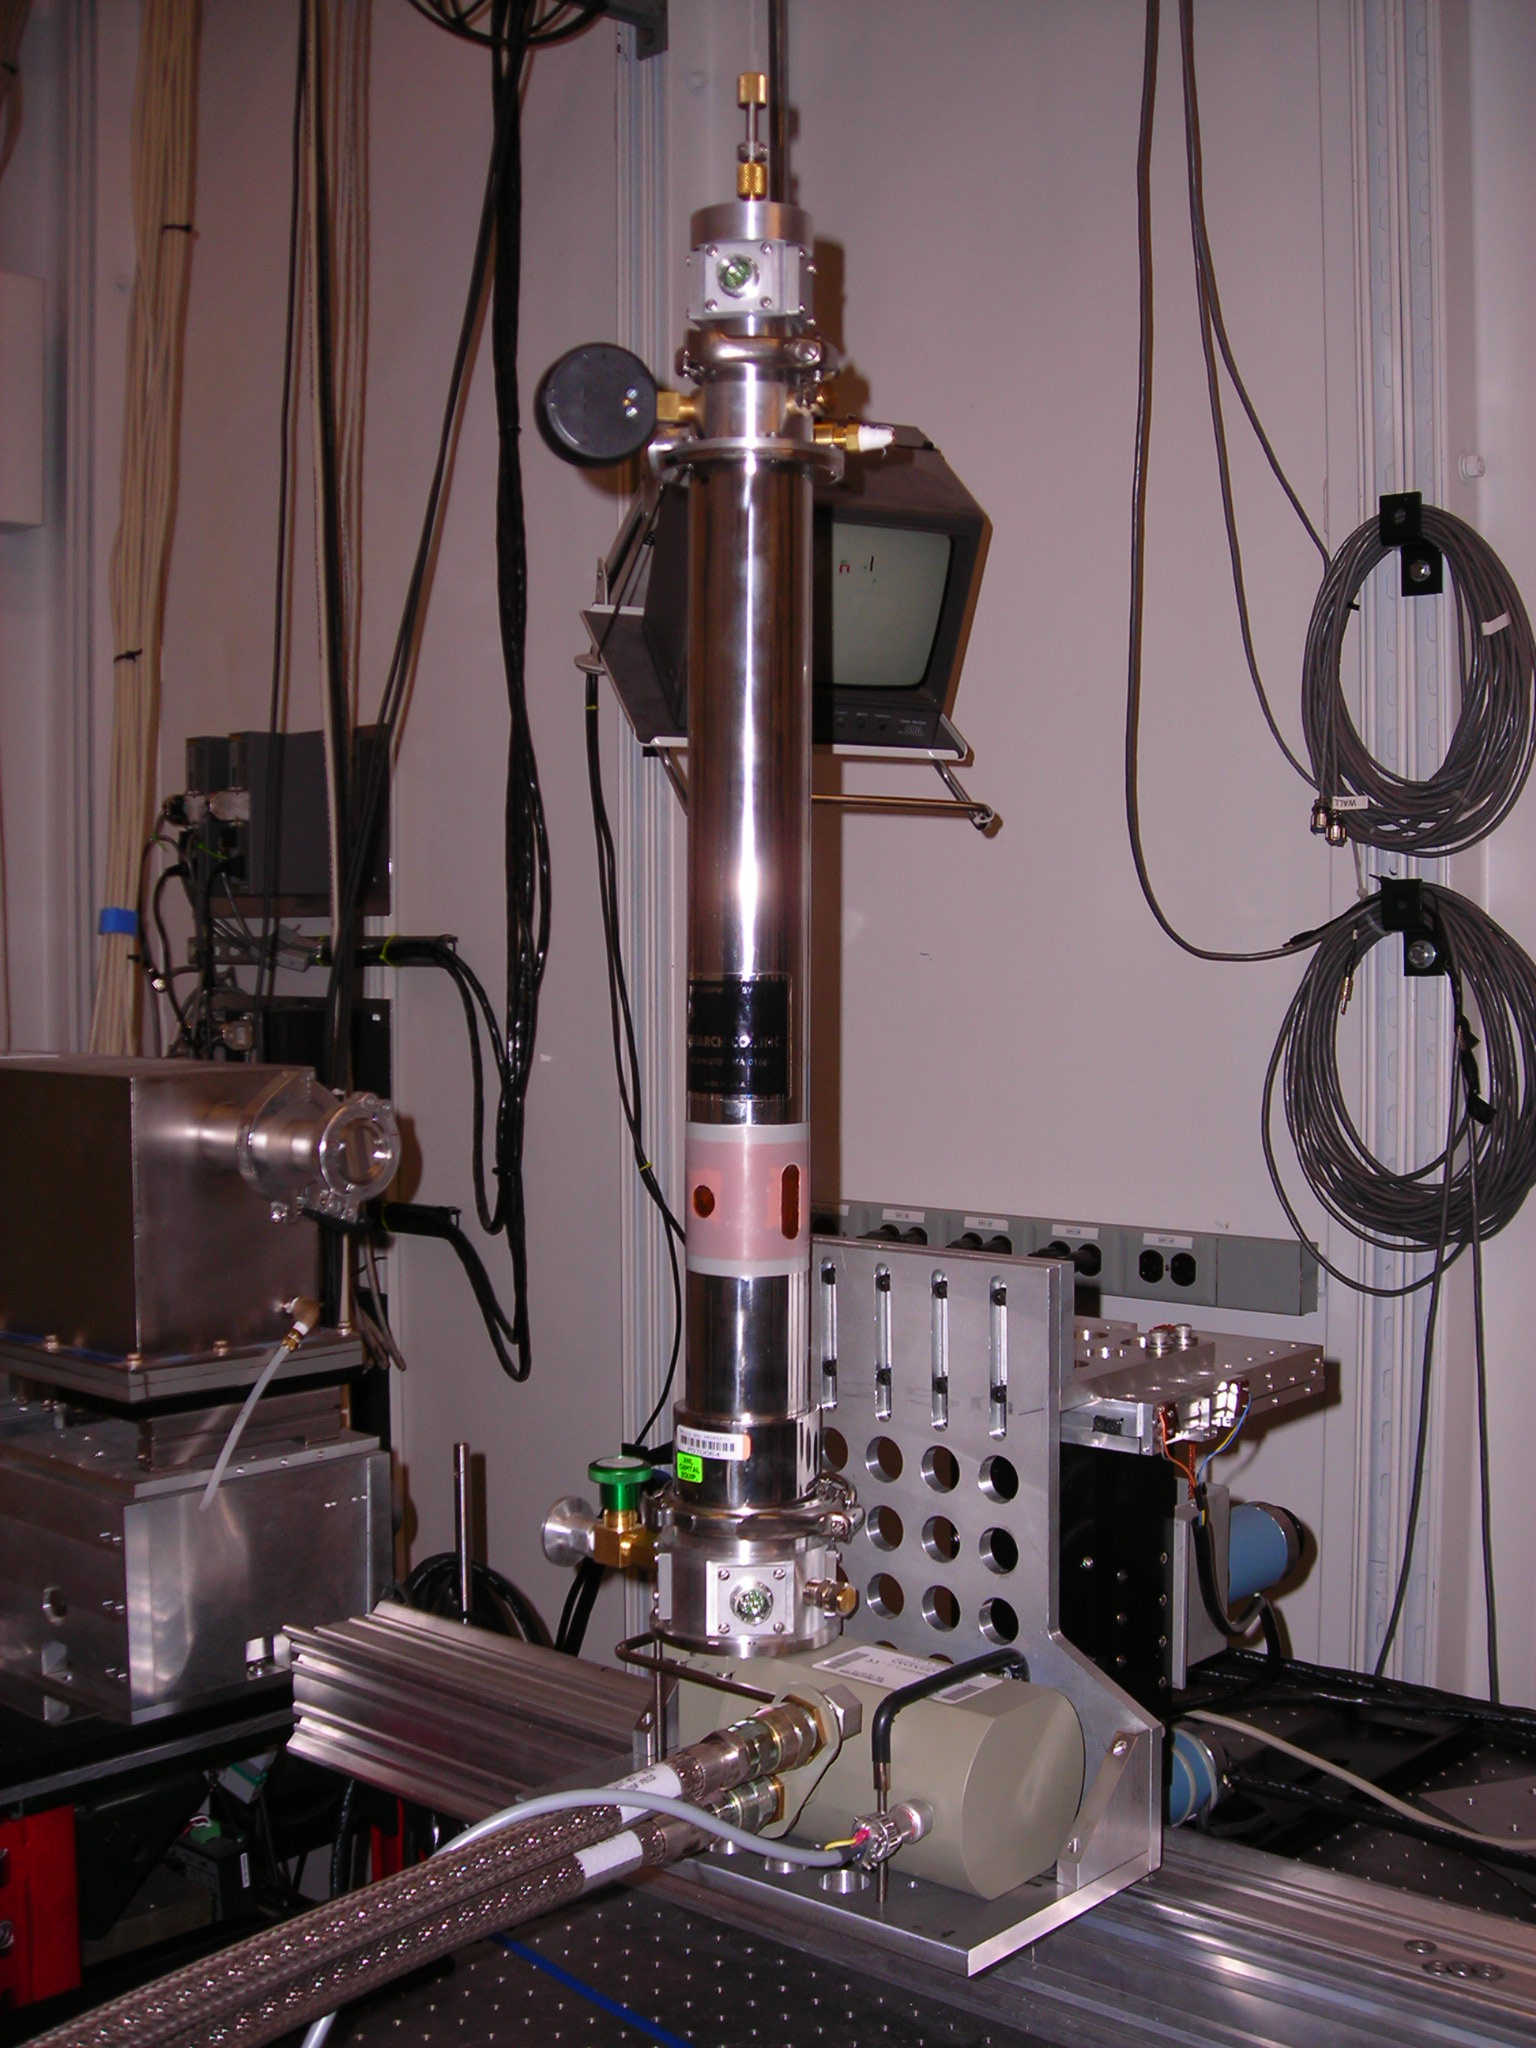
\includegraphics[width=0.8\linewidth]{images/displex.jpg}
    \end{column}
    \begin{column}{0.5\linewidth}
      The samples were packaged back at the University and were about
      15\,mm by 3\,mm.

      \bigskip

      We had to put the samples in the cryostat upright and slit the
      beam down to $\sim$1\,mm.

      \bigskip

      \begin{alertblock}<2>{Plan ahead!}
        Forgetting about the details leads to much worse data!
      \end{alertblock}
    \end{column}
  \end{columns}
\end{frame}

\begin{frame}
  \frametitle{Our main sample}
  \begin{columns}[T]
    \begin{column}{0.5\linewidth}
      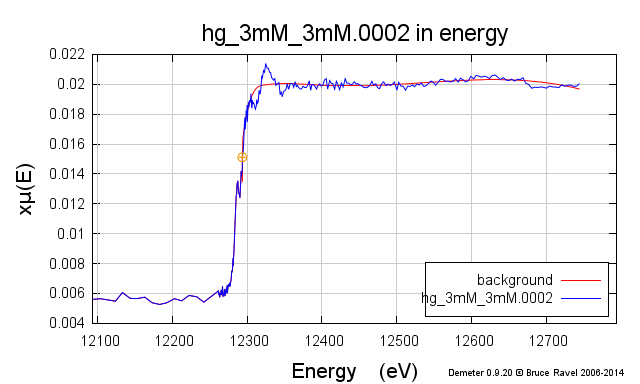
\includegraphics[width=\linewidth]{images/firstscan_e.png}

      \bigskip

      This poor data is due to low concentration, small beam, and
      large background from the As.

      \bigskip

      We measured 42 scans, taking about 22 hours.
    \end{column}
    \begin{column}{0.5\linewidth}
      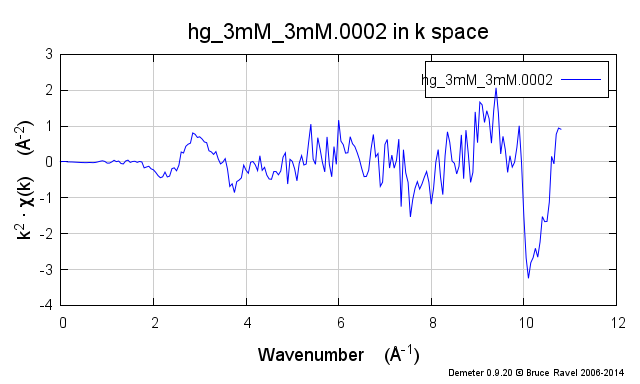
\includegraphics[width=\linewidth]{images/firstscan_k.png}

      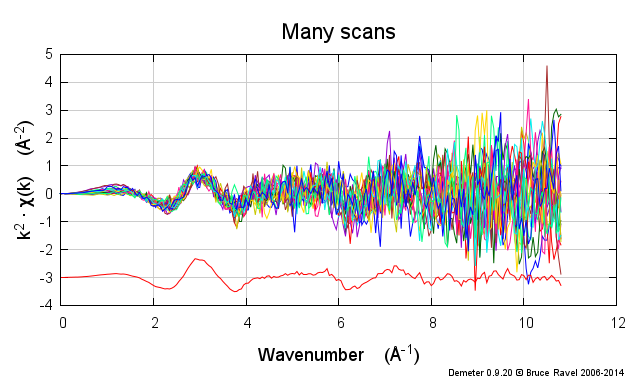
\includegraphics[width=\linewidth]{images/clt_works.png}
    \end{column}
  \end{columns}
\end{frame}


\begin{frame}
  \frametitle{Sample and control}
  \begin{columns}
    \begin{column}{0.4\linewidth}
      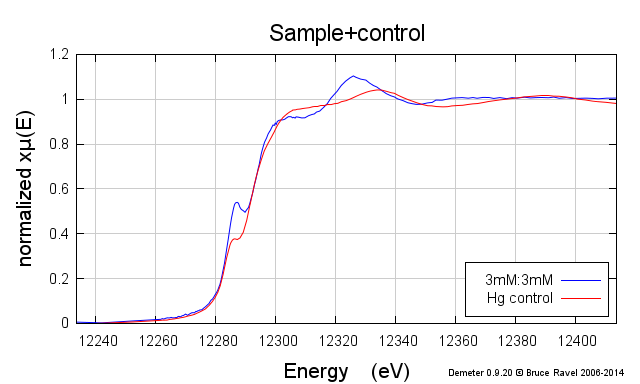
\includegraphics[width=\linewidth]{images/both_e.png}

      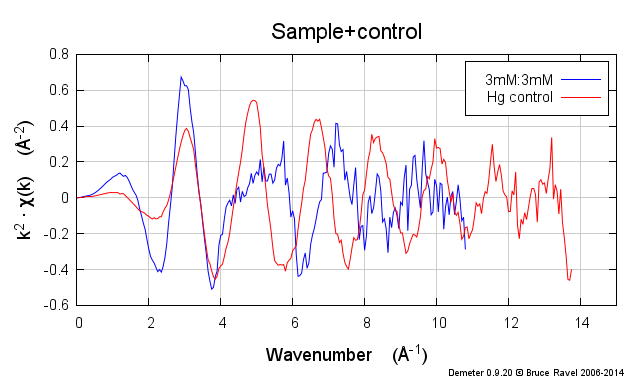
\includegraphics[width=\linewidth]{images/both_k.png}

      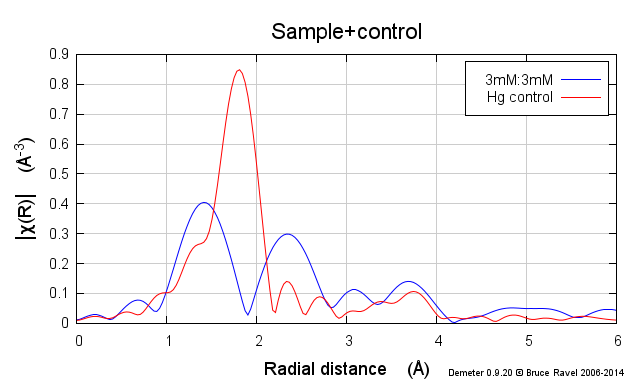
\includegraphics[width=\linewidth]{images/both_r.png}
    \end{column}
    \begin{column}{0.6\linewidth}
      Chemistry has certainly happened.

      \bigskip

      The control is clearly Hg in some kind of aqueous form.

      \bigskip

      The sample with DNA is clearly different from the control.
    \end{column}
  \end{columns}
\end{frame}

\begin{frame}
  \frametitle{Question \#1}
  \begin{exampleblock}{Is all Hg taken up by the DNA?}
    \centering To answer this, we measured a sample with excess Hg.
  \end{exampleblock}
  \begin{columns}[T]
    \begin{column}{0.5\linewidth}
      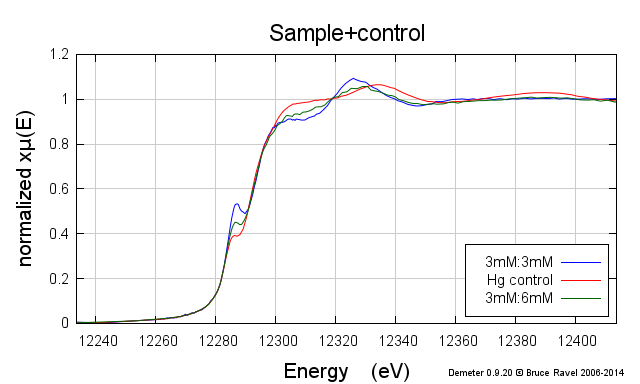
\includegraphics[width=\linewidth]{images/excess.png}

      \medskip

      Let's go do some linear combination fitting...
    \end{column}
    \begin{column}{0.5\linewidth}
      \visible<2>{
        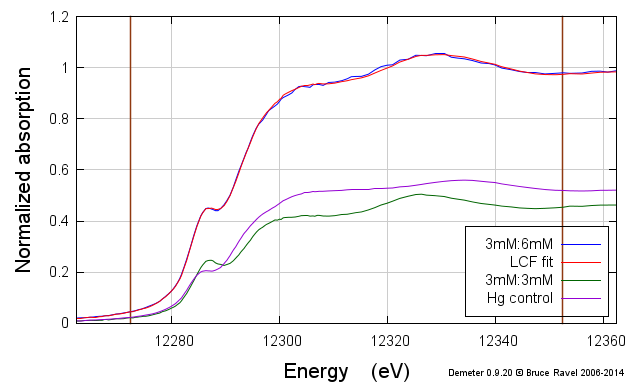
\includegraphics[width=\linewidth]{images/lcf.png}

        \medskip

        Yes, all the Hg is taken up by the DNA.\\
        47(1)\% sample + 53(1)\% control
      }
    \end{column}
  \end{columns}
\end{frame}

\section{DNA}


\begin{frame}
  \frametitle{The nucleotides}
  \begin{columns}[T]
    \begin{column}{0.5\linewidth}
      {\tiny
        \input{nucleotides/adenosinemonophosphate.chemfig}}
    \end{column}
    \begin{column}{0.5\linewidth}
      {\tiny 
        \input{nucleotides/guanisinemonophosphate.chemfig}}
    \end{column}
  \end{columns}

  \bigskip

  \begin{columns}[T]
    \begin{column}{0.5\linewidth}
      {\tiny
        \input{nucleotides/thymidinemonophosphate.chemfig}
      }     
    \end{column}
    \begin{column}{0.5\linewidth}
      {\tiny
        \input{nucleotides/cytodinemonophosphate.chemfig}
      }      
    \end{column}
  \end{columns}

  \begin{textblock*}{0.2\linewidth}(4.5\TPHorizModule,3.0\TPVertModule)%
    Adenisine
  \end{textblock*}
  \begin{textblock*}{0.2\linewidth}(17\TPHorizModule,7.0\TPVertModule)%
    Guanosine
  \end{textblock*}
  \begin{textblock*}{0.2\linewidth}(2\TPHorizModule,12.0\TPVertModule)%
    Thymidine
  \end{textblock*}
  \begin{textblock*}{0.2\linewidth}(13\TPHorizModule,13\TPVertModule)%
    Cytidine
  \end{textblock*}
  \begin{textblock*}{0.2\linewidth}(8.75\TPHorizModule,9\TPVertModule)%
    \textbf{Purines}
  \end{textblock*}
  \begin{textblock*}{0.2\linewidth}(8.5\TPHorizModule,18\TPVertModule)%
    \textbf{Pyridines}
  \end{textblock*}
  
\end{frame}

\begin{frame}
  \frametitle{2D and 3D representations}
  The 2D figures on the previous page were generated from the 
  \href{http://en.wikipedia.org/wiki/Simplified_molecular-input_line-entry_system}%
  {\color{Blue4}canonical SMILES strings}:

  \bigskip

  \begin{description}
  \item[Adenisine] {\tiny C1=NC2=C(C(=N1)N)N=CN2C3C(C(C(O3)COP(=O)(O)O)O)O}
  \item[Thymidine] {\tiny CC1=CN(C(=O)NC1=O)C2CC(C(O2)COP(=O)(O)O)O}
  \item[Guanosine] {\tiny C1=NC2=C(N1C3C(C(C(O3)COP(=O)(O)O)O)O)NC(=NC2=O)N}
  \item[Cytidine] {\tiny C1=CN(C(=O)N=C1N)C2C(C(C(O2)COP(=O)(O)O)O)O}
  \end{description}

  \bigskip

  \begin{alertblock}{}
    \centering Neat!  But we need 3D structures to run \textsc{feff}...
  \end{alertblock}
\end{frame}

\begin{frame}
  \frametitle{Structure from PubChem}
  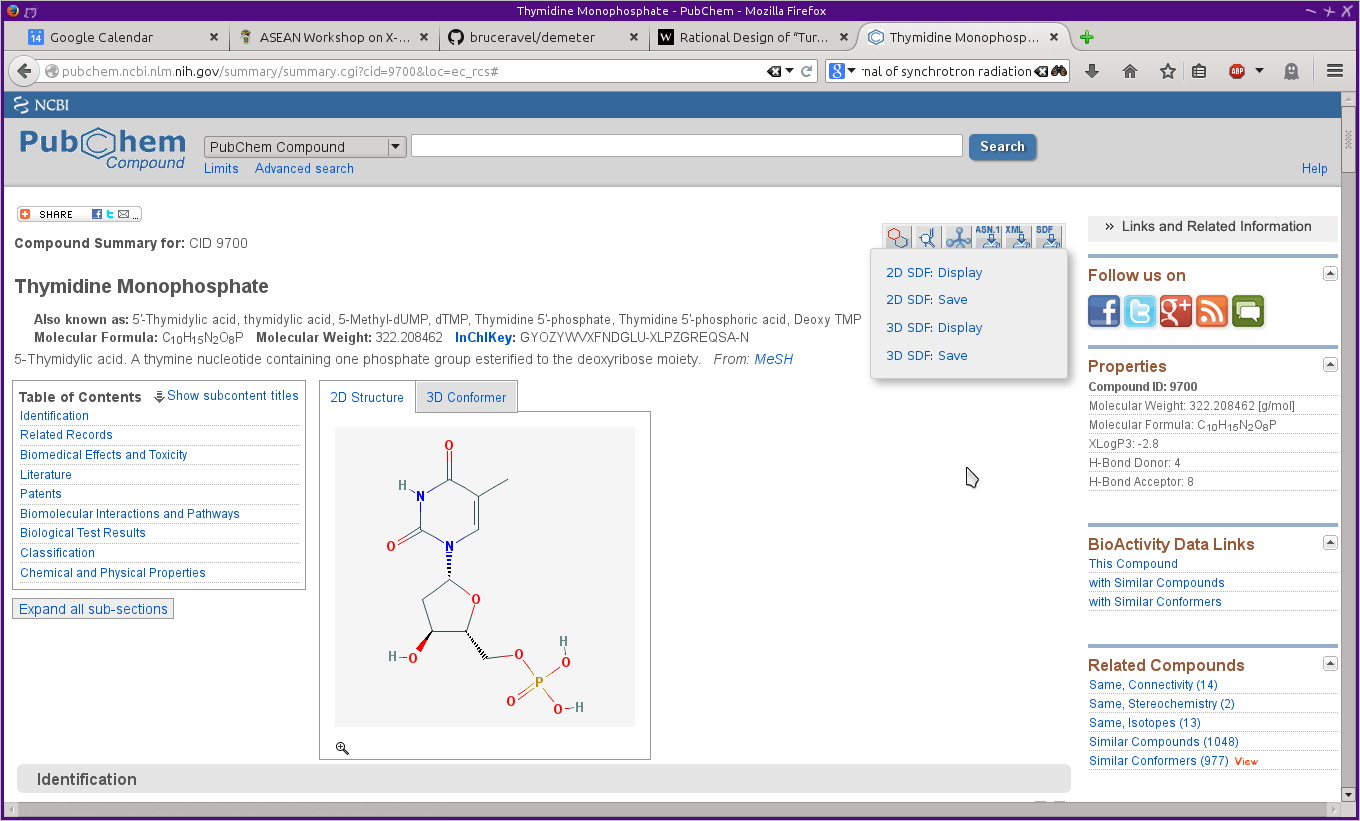
\includegraphics[width=\linewidth]{images/Thymidine-PubChem.png}  

  \medskip

  \begin{flushright}
    \href{http://pubchem.ncbi.nlm.nih.gov/}%
    {\color{Blue4}\texttt{http://pubchem.ncbi.nlm.nih.gov/}}
  \end{flushright}
\end{frame}

\begin{frame}[fragile]
  \frametitle{Cartesian coordinates: 3D SDF file}
  \begin{columns}
    \begin{column}{0.7\linewidth}
  \begin{alltt}
    \tiny
 9700
  -OEChem-05141416293D

 36 37  0     1  0  0  0  0  0999 V2000
   -3.5515   -1.5175    0.1599 P   0  0  0  0  0  0  0  0  0  0  0  0
   -0.4389    1.3396    1.0202 O   0  0  0  0  0  0  0  0  0  0  0  0
   -0.9101    4.1569   -0.0812 O   0  0  0  0  0  0  0  0  0  0  0  0
   -2.7552   -0.1874    0.6247 O   0  0  0  0  0  0  0  0  0  0  0  0
    3.6173    1.7470    0.3907 O   0  0  0  0  0  0  0  0  0  0  0  0
    3.8378   -2.8022   -0.2452 O   0  0  0  0  0  0  0  0  0  0  0  0
   -2.5475   -2.2163   -0.8977 O   0  0  0  0  0  0  0  0  0  0  0  0
   -4.7267   -0.9241   -0.7790 O   0  0  0  0  0  0  0  0  0  0  0  0
   -4.0197   -2.4002    1.2798 O   0  0  0  0  0  0  0  0  0  0  0  0
    1.6113    0.5684    0.1973 N   0  0  0  0  0  0  0  0  0  0  0  0
    3.7127   -0.5224    0.0726 N   0  0  0  0  0  0  0  0  0  0  0  0
   -1.0101    2.8736   -0.6948 C   0  0  2  0  0  0  0  0  0  0  0  0
   -1.5699    1.8660    0.2995 C   0  0  1  0  0  0  0  0  0  0  0  0
    0.3733    2.3378   -0.9829 C   0  0  0  0  0  0  0  0  0  0  0  0
    0.7701    1.7196    0.3478 C   0  0  1  0  0  0  0  0  0  0  0  0
   -2.2796    0.6993   -0.3750 C   0  0  0  0  0  0  0  0  0  0  0  0
    1.0112   -0.6708    0.0146 C   0  0  0  0  0  0  0  0  0  0  0  0
    3.0176    0.6816    0.2323 C   0  0  0  0  0  0  0  0  0  0  0  0
    1.6792   -1.8209   -0.1381 C   0  0  0  0  0  0  0  0  0  0  0  0
    3.1656   -1.7831   -0.1119 C   0  0  0  0  0  0  0  0  0  0  0  0
    1.0130   -3.1449   -0.3336 C   0  0  0  0  0  0  0  0  0  0  0  0
   -1.6278    2.9841   -1.5911 H   0  0  0  0  0  0  0  0  0  0  0  0
   -2.2303    2.3332    1.0386 H   0  0  0  0  0  0  0  0  0  0  0  0

      (plus several more hydrogen atoms)
  \end{alltt}
    \end{column}
    \begin{column}{0.3\linewidth}
      Here is the ``SDF'' file downloaded from PubChem.

      \bigskip

      Along with lots of stuff not relevant to the EXAFS analysis, we
      find the Cartesian coordinates of all the atoms in thymidine
      monophosphate!
    \end{column}
  \end{columns}

  \begin{textblock*}{0.7\linewidth}(0pt,19\TPVertModule)%%
    \tiny \href{http://en.wikipedia.org/wiki/Chemical_table_file#SDF}%
    {\color{Blue4}SDF = Structure data file}
  \end{textblock*}
\end{frame}

\begin{frame}[fragile]
  \frametitle{Cartesian coordinates: Feff input file}
  \begin{columns}
    \begin{column}{0.5\linewidth}
  \begin{alltt}
\tiny
 {\color{Green4}TITLE Hg decorating thymidine monophosphate}
 {\color{Purple2}HOLE}      1   1.0  {\color{Blue4} *  Hg L3 edge (12284 eV), S0^2}
 {\color{Blue4}*         mphase,mpath,mfeff,mchi}
 {\color{SteelBlue2}CONTROL}   1      1     1     1
 {\color{SteelBlue2}PRINT}     1      0     0     0
 {\color{Purple2}RMAX}      6.0

 {\color{Brown4}POTENTIALS}
 {\color{Blue4}*    ipot   Z  element}
        0   50   Hg
        1    8   O
        2    7   N
        3    6   C
        4   15   P
        5    1   H

 {\color{Brown4}ATOMS}
 {\color{Blue4}*   x       y       z    ipot}
   -3.5515   -1.5175    0.1599 4
   -0.4389    1.3396    1.0202 1
   -0.9101    4.1569   -0.0812 1
   -2.7552   -0.1874    0.6247 1
    3.6173    1.7470    0.3907 1
    3.8378   -2.8022   -0.2452 1
   -2.5475   -2.2163   -0.8977 1
   -4.7267   -0.9241   -0.7790 1
   -4.0197   -2.4002    1.2798 1
    1.6113    0.5684    0.1973 2
    3.7127   -0.5224    0.0726 2
   -1.0101    2.8736   -0.6948 3
   -1.5699    1.8660    0.2995 3
    0.3733    2.3378   -0.9829 3

 {\color{Blue4}*   (and so on...)}
  \end{alltt}
    \end{column}
    \begin{column}{0.5\linewidth}
      \begin{enumerate}
      \item Do some cutting and pasting
      \item Add some boilerplate for the header
      \item Make a sensible {\color{Brown4}\texttt{POTENTIALS}} list
      \end{enumerate}

      \bigskip

      And we are ready for the next step...
    \end{column}
  \end{columns}
\end{frame}


\begin{frame}
  \frametitle{Decorating thymidine with Hg}
  \chemfig{%
    % nitrogenous base begins
    C-[:330]C=[:30,,,,-]C(-[:90,,,,dash bond]Hg\qm)%
    -[:330,,,,-]N(-[:270,,,,-]C(%
    -[:210,,,,-]@{2}{\color{black!40!red}N}(-[:270,,,,dash bond]@{1}{\color{black!40!red}\underline{Hg}\qm})%
    -[:150,,,,-]@{3}C(=[:210,,,,-]O)%
    -[:90,,,,-]C)=[:330,,,,-]O(-[:330,,,,dash bond]\widetilde{Hg}\qm))%
    % sugar begins
    -[:30]C-[:84]C(-[:150,,,,dash bond]\overline{Hg}\qm)-[:12]C(-[:66,,,1]OH^{\color{white}2})%
    -[:300]C(-[:228]O(-[:285,,,,dash bond]\overline{Hg}\qm)%
    % bridge sugar to phosphate
    -[:156]C)-[:354]C-[:294]O-[:354]%
    % phosphate begins
    P(-[:54]\mcfright{O}{^{\mcfminus}})%
    (-[:294]\mcfright{O}{^{\mcfminus}}
    (-[:294,,,,dash bond]\widetilde{Hg}\qm))%
    =[:354]O%
    \namebond{2}{1}{\footnotesize $a$}
    \namebond{2}{3}{\footnotesize $b$}
    \arclabel{0.5cm}{1}{2}{3}{\footnotesize$\varphi$}
  }
\end{frame}

\end{document}

%%% Local Variables:
%%% mode: latex
%%% TeX-master: t
%%% TeX-parse-self: t
%%% TeX-auto-save: t
%%% TeX-auto-untabify: t
%%% TeX-PDF-mode: t
%%% End:
